\begin{figure}[h]
  \definecolor{c1}{RGB}{191,255,191}
  \definecolor{c2}{RGB}{127,255,127}
  \definecolor{c3}{RGB}{64,191,64}
  \definecolor{c4}{RGB}{32,127,32}
  %
  \begin{subfigure}[b]{.5\textwidth}
    \centering
    \begin{tikzpicture}
      \draw[black,ultra thick](0,0)rectangle(5,5);
      \draw[step=1cm,gray,very thin] (0,0) grid (5,5);
      \draw[black,fill=black] (4.5,4.5) circle (.4cm) node[star, star points=5,black,fill=yellow] {};
      \draw[black,fill=red] (2.5,2.5) circle (.4cm);
      \draw[vecArrow](2.5,2.5)-|(3.5,3.5)-|(4.5,4.1);
    \end{tikzpicture}
    \caption{A* Search: search through maze}
    \label{fig:a51}
    %
  \end{subfigure}
  %
  \begin{subfigure}[b]{.5\textwidth}
    \centering
    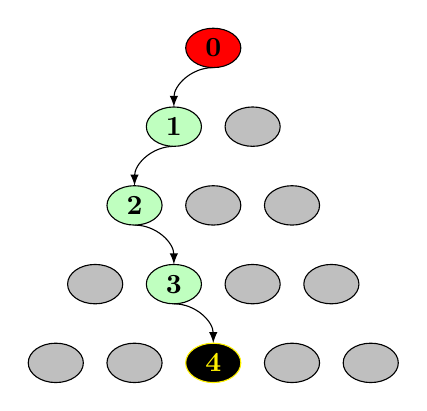
\begin{tikzpicture}[x=.5cm]
      \draw[arrows={-latex}](3,4.25) to [bend right=45] (2,3.75);
      \draw[arrows={-latex}](2,3.25) to [bend right=45] (1,2.75);
      \draw[arrows={-latex}](1,2.25) to [bend left=45] (2,1.75);
      \draw[arrows={-latex}](2,1.25) to [bend left=45] (3,0.75);
      
      \draw[black,fill=red] (3,4.5) ellipse (.35cm and .25cm) node{\textbf{0}};
      
      \draw[black,fill=c1] (2,3.5) ellipse (.35cm and .25cm) node{\textbf{1}};
      \draw[black,fill=lightgray] (4,3.5) ellipse (.35cm and .25cm);

      \draw[black,fill=c1] (1,2.5) ellipse (.35cm and .25cm) node{\textbf{2}};
      \draw[black,fill=lightgray] (3,2.5) ellipse (.35cm and .25cm);
      \draw[black,fill=lightgray] (5,2.5) ellipse (.35cm and .25cm);

      \draw[black,fill=lightgray] (0,1.5) ellipse (.35cm and .25cm);
      \draw[black,fill=c1] (2,1.5) ellipse (.35cm and .25cm) node{\textbf{3}};
      \draw[black,fill=lightgray] (4,1.5) ellipse (.35cm and .25cm);
      \draw[black,fill=lightgray] (6,1.5) ellipse (.35cm and .25cm);

      \draw[black,fill=lightgray] (-1, .5) ellipse (.35cm and .25cm);
      \draw[black,fill=lightgray] (1, .5) ellipse (.35cm and .25cm);
      \draw[yellow,fill=black] (3, .5) ellipse (.35cm and .25cm) node{\textbf{4}};
      \draw[black,fill=lightgray] (5, .5) ellipse (.35cm and .25cm);
      \draw[black,fill=lightgray] (7, .5) ellipse (.35cm and .25cm);
    \end{tikzpicture}
    \caption{A* Search: search tree, 15 nodes}
    \label{fig:a52}
    %
  \end{subfigure}


  \begin{subfigure}[b]{.5\textwidth}
    \centering
    \begin{tikzpicture}
      \draw[black,ultra thick](0,0)rectangle(5,5);
      \draw[step=1cm,gray,very thin] (0,0) grid (5,5);
      \draw[fill=darkgray] (0,1) rectangle (1,2);
      \draw[fill=darkgray] (1,4) rectangle (2,5);
      \draw[black,fill=black] (4.5,4.5) circle (.4cm) node[star, star points=5,black,fill=yellow] {};
      \draw[black,fill=red] (2.5,2.5) circle (.4cm);
      \draw[vecArrow](2.5,2.5)-|(1.5,3.7)-|(.2,4.5)-|(.8,3.7);
      \draw[vecArrow](.8,3.65)|-(.2,2.5)|-(.75,3.3);
      \draw[vecArrow](.9,3.3)-|(4.5,4.1);
    \end{tikzpicture}
    \caption{DFS: search through maze}
    \label{fig:a53}
    %
  \end{subfigure}
  %
  \begin{subfigure}[b]{.5\textwidth}
    \centering
    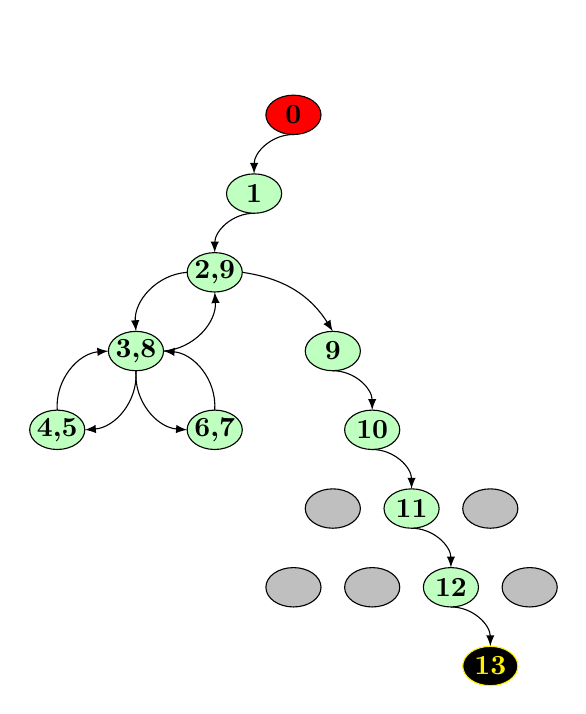
\begin{tikzpicture}
      \draw[white](0,5.5) circle(.1cm);
      \draw[arrows={-latex}](3,4.25) to [bend right=45] (2.5,3.75);%0-1
      \draw[arrows={-latex}](2.5,3.25) to [bend right=45] (2,2.75);%1-2
      \draw[arrows={-latex}](1.65,2.5) to [bend right=45] (1,1.75); %2-3
      \draw[arrows={-latex}](1,1.25)  to [bend left=45] (0.35,.5);  %3-4,5
      \draw[arrows={-latex}](0.0,0.75) to [bend left=45]  (.65,1.5); %4,5-3
      \draw[arrows={-latex}](1,1.25) to [bend right=45]  (1.65,.5);   %3-6,7
      \draw[arrows={-latex}](2,.75) to [bend right=45]  (1.35,1.5);  %6,7-3
      \draw[arrows={-latex}](1.35,1.5) to [bend right=45]  (2,2.25);  %3-2
      \draw[arrows={-latex}](2.35,2.5) to [bend left=25] (3.5,1.75);  %2-8
      \draw[arrows={-latex}] (3.5,1.25) to [bend left=45] (4,.75);%8-9
      \draw[arrows={-latex}] (4,.25) to [bend left=45] (4.5,-.25);%9-10
      \draw[arrows={-latex}] (4.5,-.75) to [bend left=45] (5,-1.25);%10-11
      \draw[arrows={-latex}] (5,-1.75) to [bend left=45] (5.5,-2.25);%11-12
      
      \draw[black,fill=red] (3,4.5) ellipse (.35cm and .25cm) node{\textbf{0}};      
      \draw[black,fill=c1] (2.5,3.5) ellipse (.35cm and .25cm) node{\textbf{1}};
      \draw[black,fill=c1] (2,2.5) ellipse (.35cm and .25cm) node{\textbf{2,9}};
      \draw[black,fill=c1] (1,1.5) ellipse (.35cm and .25cm) node{\textbf{3,8}};
      \draw[black,fill=c1] (0,0.5) ellipse (.35cm and .25cm) node{\textbf{4,5}};
      \draw[black,fill=c1] (2,0.5) ellipse (.35cm and .25cm) node{\textbf{6,7}};
      \draw[black,fill=c1] (3.5,1.5) ellipse (.35cm and .25cm) node{\textbf{9}};
      \draw[black,fill=c1] (4,0.5) ellipse (.35cm and .25cm) node{\textbf{10}};
      \draw[black,fill=c1] (4.5,-.5) ellipse (.35cm and .25cm) node{\textbf{11}};
      \draw[black,fill=lightgray] (3.5,-.5) ellipse (.35cm and .25cm) node{\textbf{}};
      \draw[black,fill=lightgray] (5.5,-.5) ellipse (.35cm and .25cm) node{\textbf{}};
      \draw[black,fill=c1] (5,-1.5) ellipse (.35cm and .25cm) node{\textbf{12}};
      \draw[black,fill=lightgray] (4,-1.5) ellipse (.35cm and .25cm) node{\textbf{}};
      \draw[black,fill=lightgray] (3,-1.5) ellipse (.35cm and .25cm) node{\textbf{}};
      \draw[black,fill=lightgray] (6,-1.5) ellipse (.35cm and .25cm) node{\textbf{}};
      \draw[yellow,fill=black] (5.5, -2.5) ellipse (.35cm and .25cm) node{\textbf{13}};
    \end{tikzpicture}
    \caption{DFS: search tree, 16 nodes}
    \label{fig:a54}
    %
  \end{subfigure}

  %
  \begin{subfigure}[b]{.4\textwidth}
    \centering
    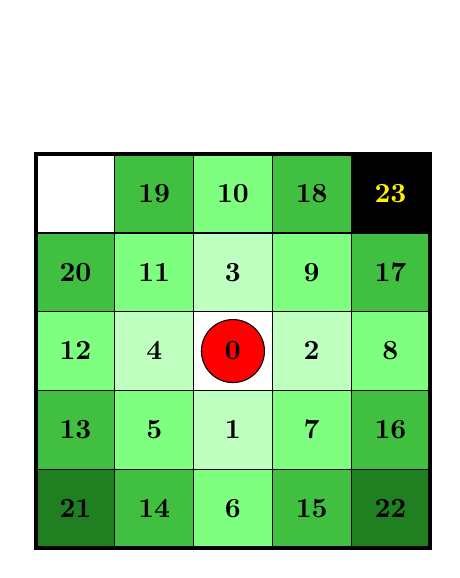
\begin{tikzpicture}
      \draw[white](0,6.5) circle(.1cm);
      \draw[step=1cm,gray,very thin] (0,0) grid (5,5);
      
      \draw[fill=c4]   (0,0)rectangle(1,1) node[pos=.5] {\textbf{21}};      
      \draw[fill=c3]   (1,0)rectangle(2,1) node[pos=.5] {\textbf{14}};      
      \draw[fill=c2]   (2,0)rectangle(3,1) node[pos=.5] {\textbf{6}};      
      \draw[fill=c3]   (3,0)rectangle(4,1) node[pos=.5] {\textbf{15}};      
      \draw[fill=c4]   (4,0)rectangle(5,1) node[pos=.5] {\textbf{22}};      
      \draw[fill=c3]   (0,1)rectangle(1,2) node[pos=.5] {\textbf{13}};      
      \draw[fill=c2]   (1,1)rectangle(2,2) node[pos=.5] {\textbf{5}};      
      \draw[fill=c1]   (2,1)rectangle(3,2) node[pos=.5] {\textbf{1}};      
      \draw[fill=c2]   (3,1)rectangle(4,2) node[pos=.5] {\textbf{7}};      
      \draw[fill=c3]   (4,1)rectangle(5,2) node[pos=.5] {\textbf{16}};      
      \draw[fill=c2]   (0,2)rectangle(1,3) node[pos=.5] {\textbf{12}};      
      \draw[fill=c1]   (1,2)rectangle(2,3) node[pos=.5] {\textbf{4}};      
      \draw[fill=white](2,2)rectangle(3,3) node[pos=.5] {\textbf{0}};      
      \draw[fill=c1]   (3,2)rectangle(4,3) node[pos=.5] {\textbf{2}};      
      \draw[fill=c2]   (4,2)rectangle(5,3) node[pos=.5] {\textbf{8}};      
      \draw[fill=c3]   (0,3)rectangle(1,4) node[pos=.5] {\textbf{20}};      
      \draw[fill=c2]   (1,3)rectangle(2,4) node[pos=.5] {\textbf{11}};      
      \draw[fill=c1]   (2,3)rectangle(3,4) node[pos=.5] {\textbf{3}};      
      \draw[fill=c2]   (3,3)rectangle(4,4) node[pos=.5] {\textbf{9}};      
      \draw[fill=c3]   (4,3)rectangle(5,4) node[pos=.5] {\textbf{17}};      
      \draw[fill=white](0,4)rectangle(1,5) node[pos=.5] {\textbf{}};      
      \draw[fill=c3]   (1,4)rectangle(2,5) node[pos=.5] {\textbf{19}};      
      \draw[fill=c2]   (2,4)rectangle(3,5) node[pos=.5] {\textbf{10}};      
      \draw[fill=c3]   (3,4)rectangle(4,5) node[pos=.5] {\textbf{18}};      
      \draw[fill=c4]   (4,4)rectangle(5,5) node[pos=.5] {\textbf{23}};      

      \draw[black,fill=red] (2.5,2.5) circle (.4cm) node{\textbf{0}};
      \draw[black,ultra thick](0,0)rectangle(5,5);
      \draw[black,fill=black] (4,4) rectangle (5,5) node[pos=.5,yellow] {\textbf{23}};

    \end{tikzpicture}
    \caption{BFS: search tree, 24 nodes}
    \label{fig:a55}
    %
  \end{subfigure}
  %
  \begin{subfigure}[b]{.6\textwidth}
    \centering
    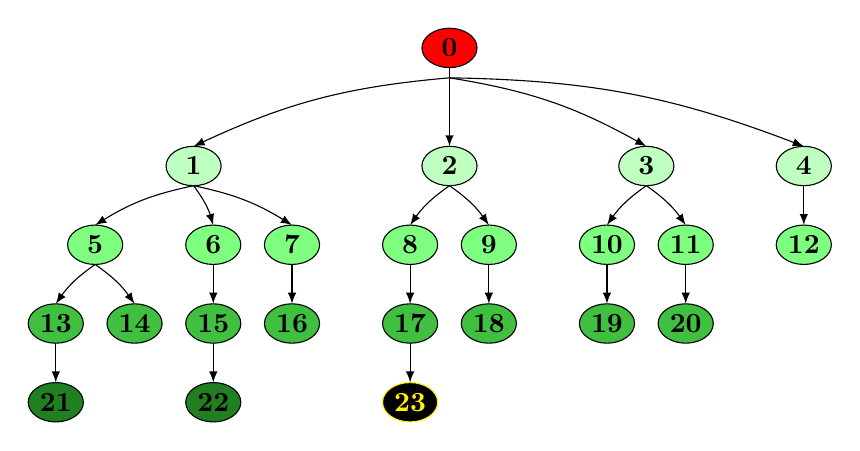
\begin{tikzpicture}[x=1.0cm]
      \draw[black,fill=red] (6,4.5) ellipse (.35cm and .25cm) node {\textbf{0}};

      \draw[black,fill=c1] (2.75, 3) ellipse (.35cm and .25cm) node {\textbf{1}};
      \draw[black,fill=c1] (6, 3) ellipse (.35cm and .25cm) node {\textbf{2}};
      \draw[black,fill=c1] (8.50, 3) ellipse (.35cm and .25cm) node {\textbf{3}};
      \draw[black,fill=c1] (10.5, 3) ellipse (.35cm and .25cm) node {\textbf{4}};

      \draw[black,fill=c2] (1.5, 2) ellipse (.35cm and .25cm) node {\textbf{5}};
      \draw[black,fill=c2] (3.0, 2) ellipse (.35cm and .25cm) node {\textbf{6}};
      \draw[black,fill=c2] (4.0, 2) ellipse (.35cm and .25cm) node {\textbf{7}};
      \draw[black,fill=c2] (5.5, 2) ellipse (.35cm and .25cm) node {\textbf{8}};
      \draw[black,fill=c2] (6.5, 2) ellipse (.35cm and .25cm) node {\textbf{9}};
      \draw[black,fill=c2] (8.0, 2) ellipse (.35cm and .25cm) node {\textbf{10}};
      \draw[black,fill=c2] (9.0, 2) ellipse (.35cm and .25cm) node {\textbf{11}};
      \draw[black,fill=c2] (10.5,2) ellipse (.35cm and .25cm) node {\textbf{12}};

      \draw[black,fill=c3] (1.0, 1) ellipse (.35cm and .25cm) node {\textbf{13}};
      \draw[black,fill=c3] (2.0, 1) ellipse (.35cm and .25cm) node {\textbf{14}};
      \draw[black,fill=c3] (3.0, 1) ellipse (.35cm and .25cm) node {\textbf{15}};
      \draw[black,fill=c3] (4.0, 1) ellipse (.35cm and .25cm) node {\textbf{16}};
      \draw[black,fill=c3] (5.5, 1) ellipse (.35cm and .25cm) node {\textbf{17}};
      \draw[black,fill=c3] (6.5, 1) ellipse (.35cm and .25cm) node {\textbf{18}};
      \draw[black,fill=c3] (8.0, 1) ellipse (.35cm and .25cm) node {\textbf{19}};
      \draw[black,fill=c3] (9.0, 1) ellipse (.35cm and .25cm) node {\textbf{20}};

      \draw[black,fill=c4] ( 1, 0) ellipse (.35cm and .25cm) node {\textbf{21}};
      \draw[black,fill=c4] ( 3, 0) ellipse (.35cm and .25cm) node {\textbf{22}};
      \draw[yellow,fill=black] (5.5, 0) ellipse (.35cm and .25cm) node {\textbf{23}};

      \draw (6,4.25) to (6,4.12);
      \draw[arrows={-latex}] (6,4.12) to [bend right=10] (2.75,3.25);
      \draw[arrows={-latex}] (6,4.12) to (6,3.25);
      \draw[arrows={-latex}] (6,4.12) to [bend left=10] (8.5,3.25);
      \draw[arrows={-latex}] (6,4.12) to [bend left=10] (10.5,3.25);

      \draw[arrows={-latex}] (2.75,2.75) to [bend right=10] (1.5,2.25);
      \draw[arrows={-latex}] (2.75,2.75) to [bend left=10]  (3,2.25);
      \draw[arrows={-latex}] (2.75,2.75) to [bend left=10]  (4,2.25);

      \draw[arrows={-latex}] (6,2.75) to [bend right=10] (5.5,2.25);
      \draw[arrows={-latex}] (6,2.75) to [bend left=10]  (6.5,2.25);

      \draw[arrows={-latex}] (8.5,2.75) to [bend right=10] (8,2.25);
      \draw[arrows={-latex}] (8.5,2.75) to [bend left=10]  (9,2.25);

      \draw[arrows={-latex}] (10.5,2.75) to (10.5,2.25);

      \draw[arrows={-latex}] (1.5,1.75) to [bend right=10] (1,1.25);
      \draw[arrows={-latex}] (1.5,1.75) to [bend left=10]  (2,1.25);

      \draw[arrows={-latex}] (3,1.75) to (3,1.25);

      \draw[arrows={-latex}] (4,1.75) to (4,1.25);

      \draw[arrows={-latex}] (5.5,1.75) to (5.5,1.25);

      \draw[arrows={-latex}] (6.5,1.75) to (6.5,1.25);

      \draw[arrows={-latex}] (8,1.75) to (8,1.25);

      \draw[arrows={-latex}] (9,1.75) to (9,1.25);

      \draw[arrows={-latex}] (1,0.75) to (1,0.25);

      \draw[arrows={-latex}] (3,0.75) to (3,0.25);

      \draw[arrows={-latex}] (5.5,0.75) to (5.5,0.25);




      
    \end{tikzpicture}
    \caption{BFS: search tree}
    \label{fig:a56}
    %
  \end{subfigure}

    
\end{figure}
